\documentclass{beamer}
\usepackage[utf8]{inputenc}
\usepackage[spanish]{babel}
\usepackage{amsmath}
\usepackage{amsfonts}
\usepackage{amssymb}
\usepackage{amsthm}

\graphicspath{ {Figures/} }

%\usetheme{AnnArbor}
%\usetheme{Antibes}
%\usetheme{Bergen}
%\usetheme{Berkeley}
%\usetheme{Berlin}
%\usetheme{Boadilla}
%\usetheme{boxes}
%\usetheme{CambridgeUS}
%\usetheme{Copenhagen}
%\usetheme{Darmstadt}
%\usetheme{default}
%\usetheme{Frankfurt}
%\usetheme{Goettingen}
%\usetheme{Hannover}
%\usetheme{Ilmenau}
%\usetheme{JuanLesPins}
%\usetheme{Luebeck}
\usetheme{Madrid}
%\usetheme{Malmoe}
%\usetheme{Marburg}
%\usetheme{Montpellier}
%\usetheme{PaloAlto}
%\usetheme{Pittsburgh}
%\usetheme{Rochester}
%\usetheme{Singapore}
%\usetheme{Szeged}
%\usetheme{Warsaw}

\title[Teorema de Radó]{Triangulación de superficies\\topológicas: Teorema de Radó}

\subtitle{}

\author[Jesús Bueno]{Jesús Bueno Urbano}

\institute[Universidad de Granada]{Grado en Matemáticas\\Universidad de Granada}

\date{}

\AtBeginSubsection[]
{
  \begin{frame}<beamer>{Outline}
    \tableofcontents[currentsection,currentsubsection]
  \end{frame}
}

\begin{document}

\begin{frame}
  \titlepage
\end{frame}

\section*{Motivación y preliminares}

\begin{frame}{Motivación y preliminares}
	\begin{block}{}
		Cuando un topólogo es invitado a dar una conferencia, o a escribir unas líneas sobre el significado de la Topología, no es raro que comience hablando de toros y de tazas de café; de superficies y de bandas de Möbius; de botellas de Klein y planos proyectivos; y tal vez coja una cuerda y comience a mostrarnos prácticamente la teoría de nudos. Pero el mismo topólogo, una vez en clase, no dirá nada de eso, y partiendo de un método axiomático, frío y duro como un trozo de acero, nos hablará de entornos, de abiertos, de espacios conexos, de compactificaciones, de redes, etc.
	\end{block}
\end{frame}

\begin{frame}{Motivación y preliminares}
\begin{figure}[h]
\centering
\begin{minipage}[c]{\textwidth}
\centering
    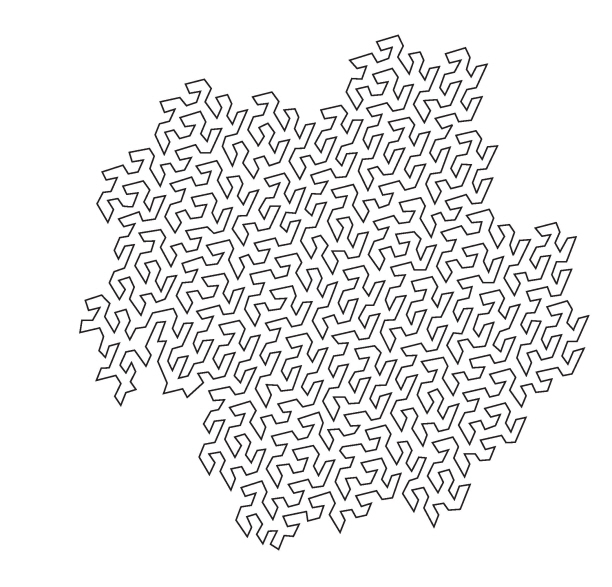
\includegraphics[]{jordancurve.jpg}
    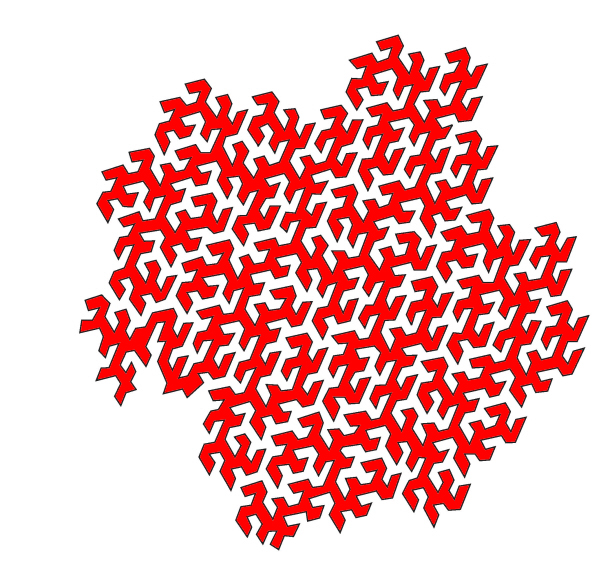
\includegraphics[]{jordancurve2.jpg}
\end{minipage}
\end{figure}
\end{frame}

\begin{frame}{Motivación y preliminares}
	\begin{block}{Teorema de la curva de Jordan}
	Sea C una curva de Jordan entonces $\mathbb{R}^2 \backslash C$ tiene exactamente dos regiones, ambas con C como frontera.
	\end{block}
	\pause
    \begin{block}{Teorema de Jordan-Schönflies}
	Sea $f$ un homeomorfismo de una curva de Jordan $C$ en otra curva curva de Jordan $C'$. Entonces $f$ puede ser extendido a un homeorfismo $F$ de todo el plano.
	\end{block}
	\pause
	\begin{block}{Teorema}
	Sean $\Gamma$ y $\Gamma'$ grafos planos biconexos tales que $g$ sea un homeomorfismo y un plano-isomorfismo de $\Gamma$ en $\Gamma'$. Entonces $g$ puede ser extendido a un homeomorfismo de todo el plano.
	\end{block}
\end{frame}

\begin{frame}{Motivación y preliminares}
    \begin{alertblock}{Definición}
	Si $C$ y $C'$ son curvas de Jordan y $\Gamma$ y $\Gamma'$ son grafos biconexos que consisten en $C$ (respectivamente $C'$) y arcos   simples en $\overline{Int}(C)$ (respectivamente $\overline{Int}(C')$), entonces $\Gamma$ y $\Gamma'$ se dice que son plano-isomorfos si existe un isomorfismo de $\Gamma$ en $\Gamma'$ cumpliendo 
\begin{enumerate}
	\item Un ciclo en $\Gamma$ es la frontera de una cara de $\Gamma$     $\iff$ La imagen del ciclo por el isomorfismo es la frontera de una cara de $\Gamma'$.
	\item La imagen por el isomorfismo del ciclo exterior de $\Gamma$ (véase $C$) es el ciclo exterior de $\Gamma'$ (véase $C'$).
\end{enumerate}
	\end{alertblock}
\end{frame}

\section*{Teorema de Radó}

\begin{frame}{Teorema de Radó}
    \begin{alertblock}{Definición}
    Una superficie $S \neq \emptyset$ es un espacio topológico que cumple que $\forall x \in S \exists V \subseteq S$ abierto con $x \in V$ y un homeomorfismo $\Phi : V \rightarrow U$ con $U$ un abierto de $\mathbb{R}^2$.A cada par $(V,\Phi)$ lo llamaremos carta local o sistema de coordenadas de $S$.
    \end{alertblock}
    \pause
    \begin{block}{Nota}
	Impondremos que $S$ sea Hausdorff y que cumpla el II Axioma de Numerabilidad.
	\end{block}
\end{frame}

\begin{frame}{Teorema de Radó}
    Consideremos ahora una colección $X$ de polígonos convexos dos a dos, junto con sus respectivos interiores, en el plano euclídeo tal que todas sus aristas son de longitud uno. Definamos un espacio topológico $S$ identificando cada arista de un polígono de $X$  con una  arista de otro, o del mismo, polígono. Está claro que el espacio identificación $S$, con la topología cociente inducida por la proyección natural $\pi\colon X\to S$,  es compacto. Además $S$ contiene de forma natural como subespacio el grafo $G$ con  vértices la proyección de las esquinas de los polígonos de $X$ y como aristas la proyección de los lados de los polígonos de $X$.
\end{frame}

\begin{frame}{Teorema de Radó}
    \begin{block}{Lema}
    El espacio topológico $S$ es una superficie si y sólo si $S$ es conexo y además es localmente homeomorfo a un disco en cada vértice de $G$.
    \\ Diremos que el grafo $G$ es un embebimiento bicelular en $S$, es decir, que éste es un grafo embebido y además cada una de sus caras es homeomorfa a un disco abierto.
    \end{block}
    \pause
    \begin{alertblock}{Definición}
    Si todos los polígonos son triángulos, entonces decimos que $G$ es una triangulación de $S$ y que $S$ es una superficie triangulable.
    \end{alertblock}
\end{frame}

\begin{frame}{Teorema de Radó}
    \begin{block}{Teorema de Radó}
    Toda superficie $S$ es homeomorfa a una superficie triangulable.
    \end{block}
\end{frame}

\begin{frame}{Teorema de Radó}
    \begin{figure}[h]
    \centering
        \begin{minipage}[c]{\textwidth}
        \centering
        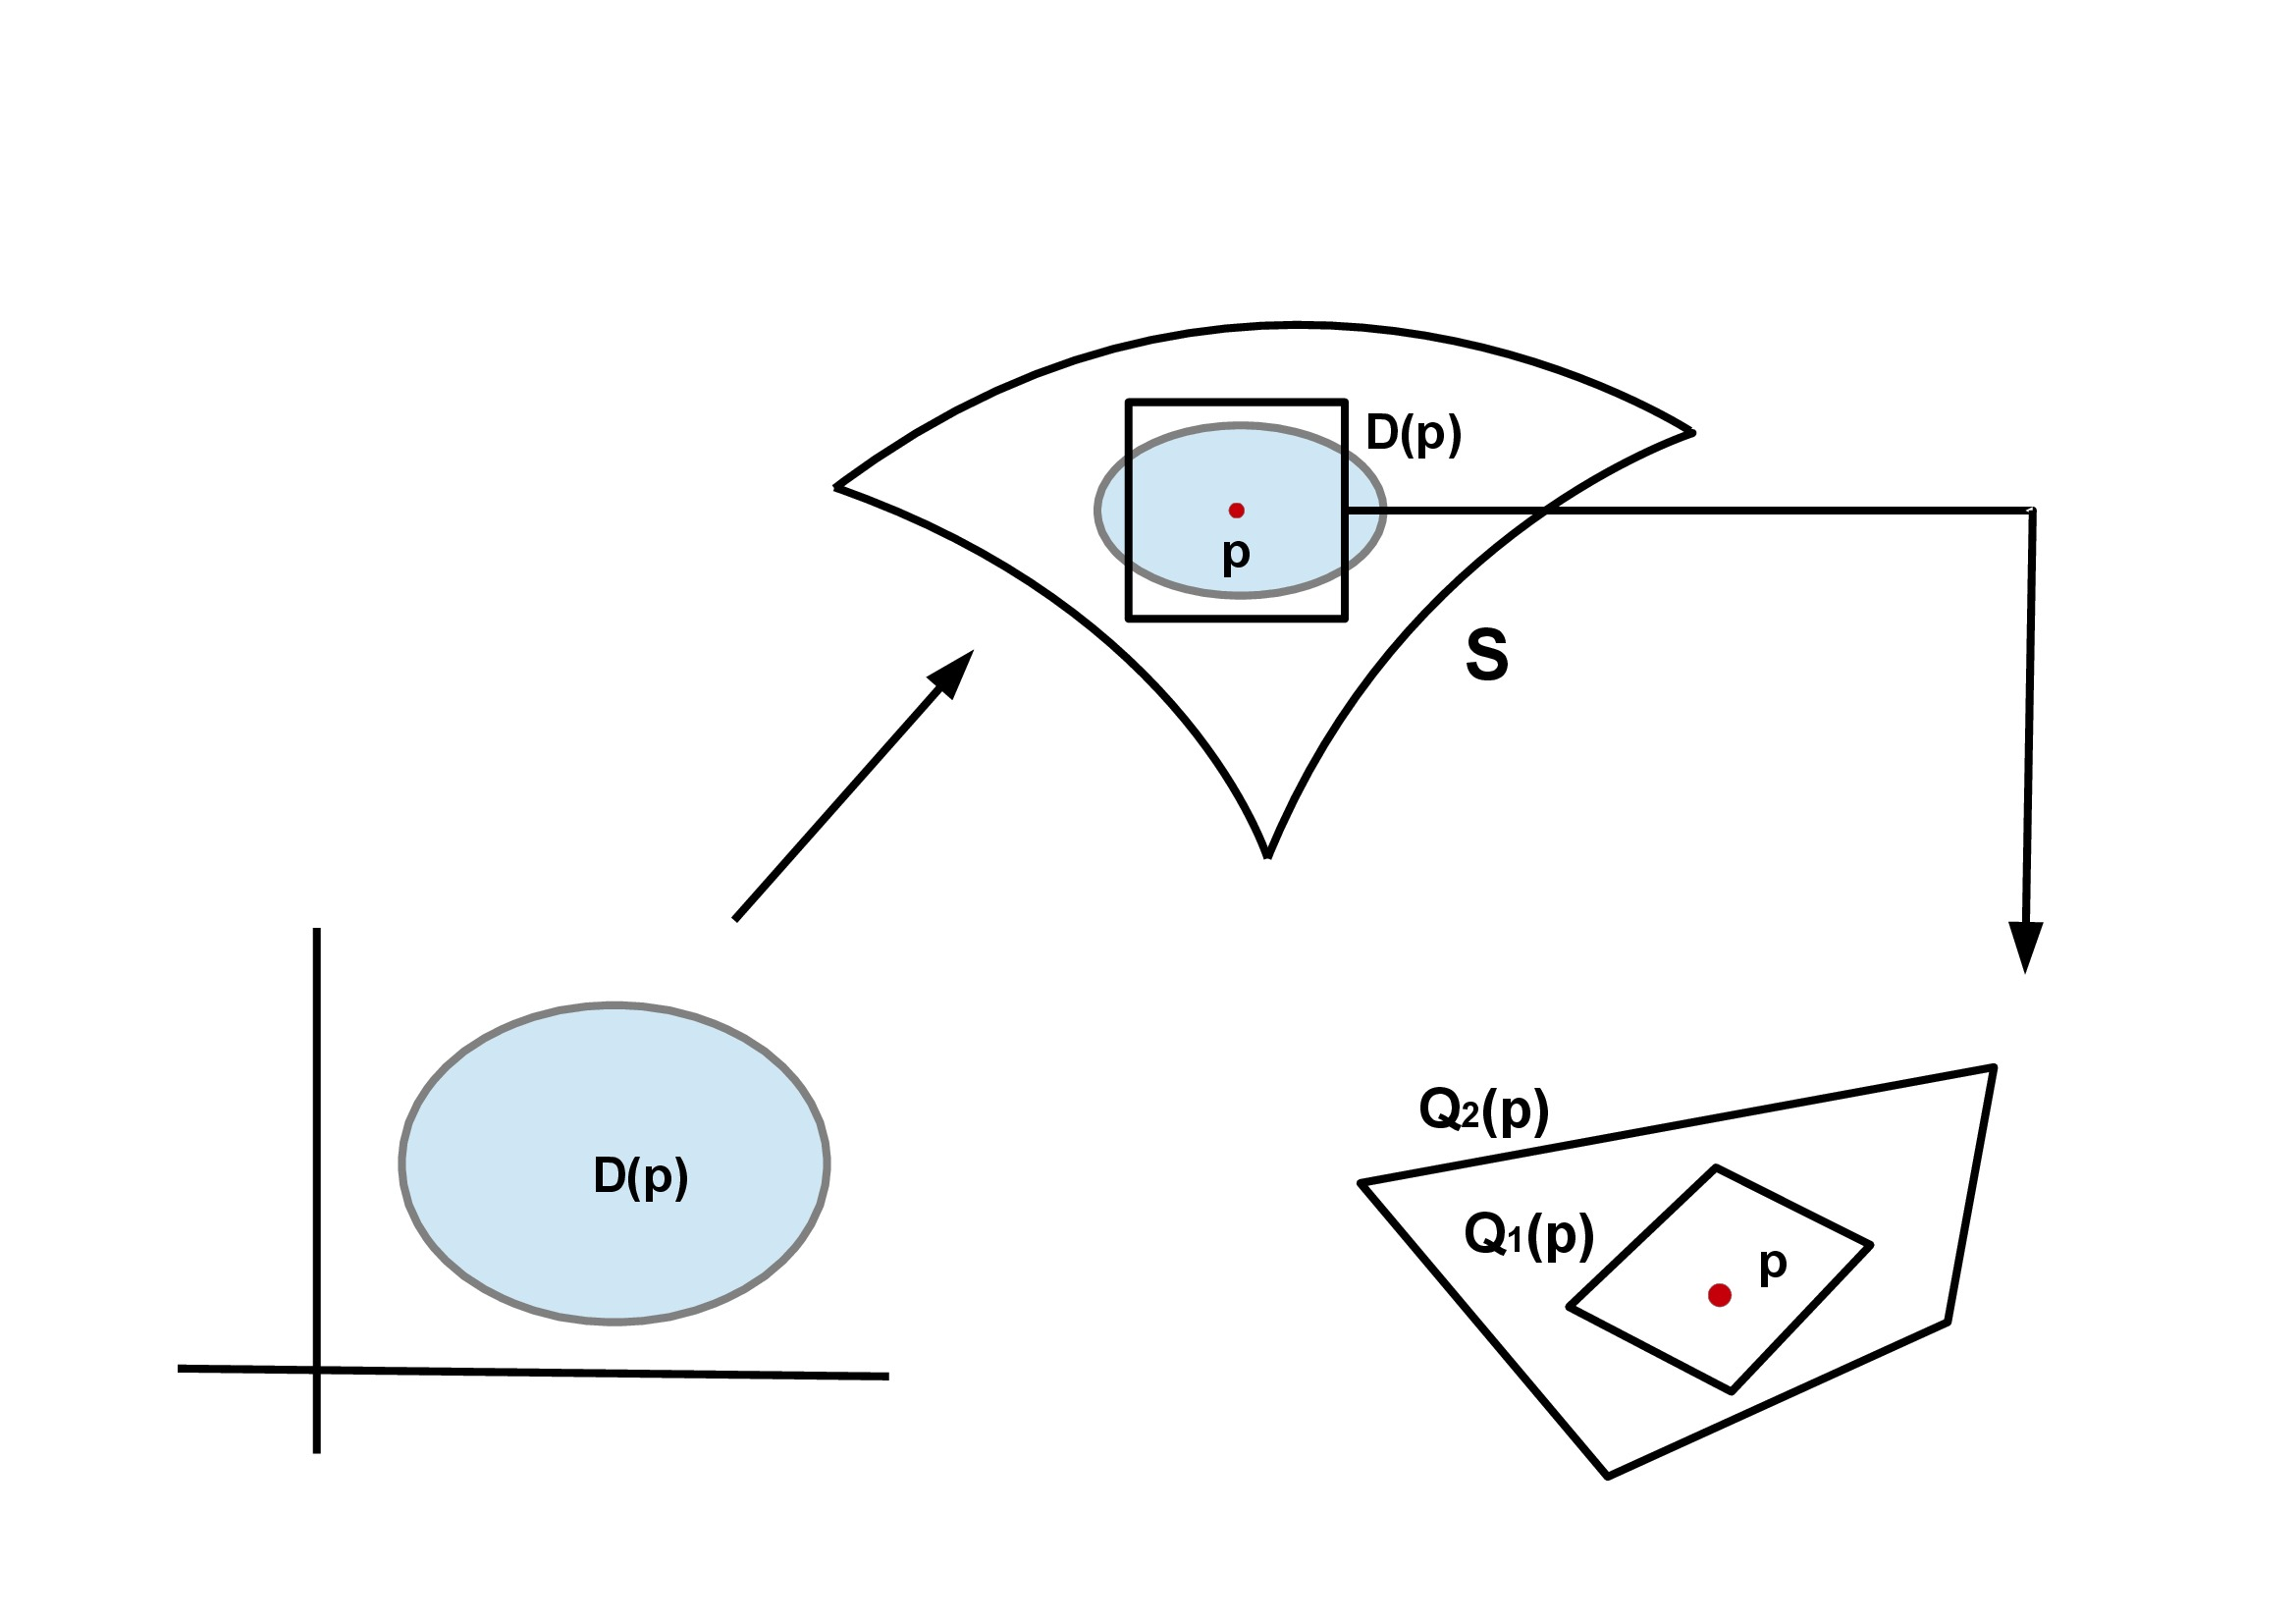
\includegraphics[width=10.0cm]{pic1.jpg}
        \end{minipage}
    \end{figure}    
\end{frame}

\begin{frame}{Teorema de Radó}
    \begin{figure}[h]
    \centering
        \begin{minipage}[c]{\textwidth}
        \centering
        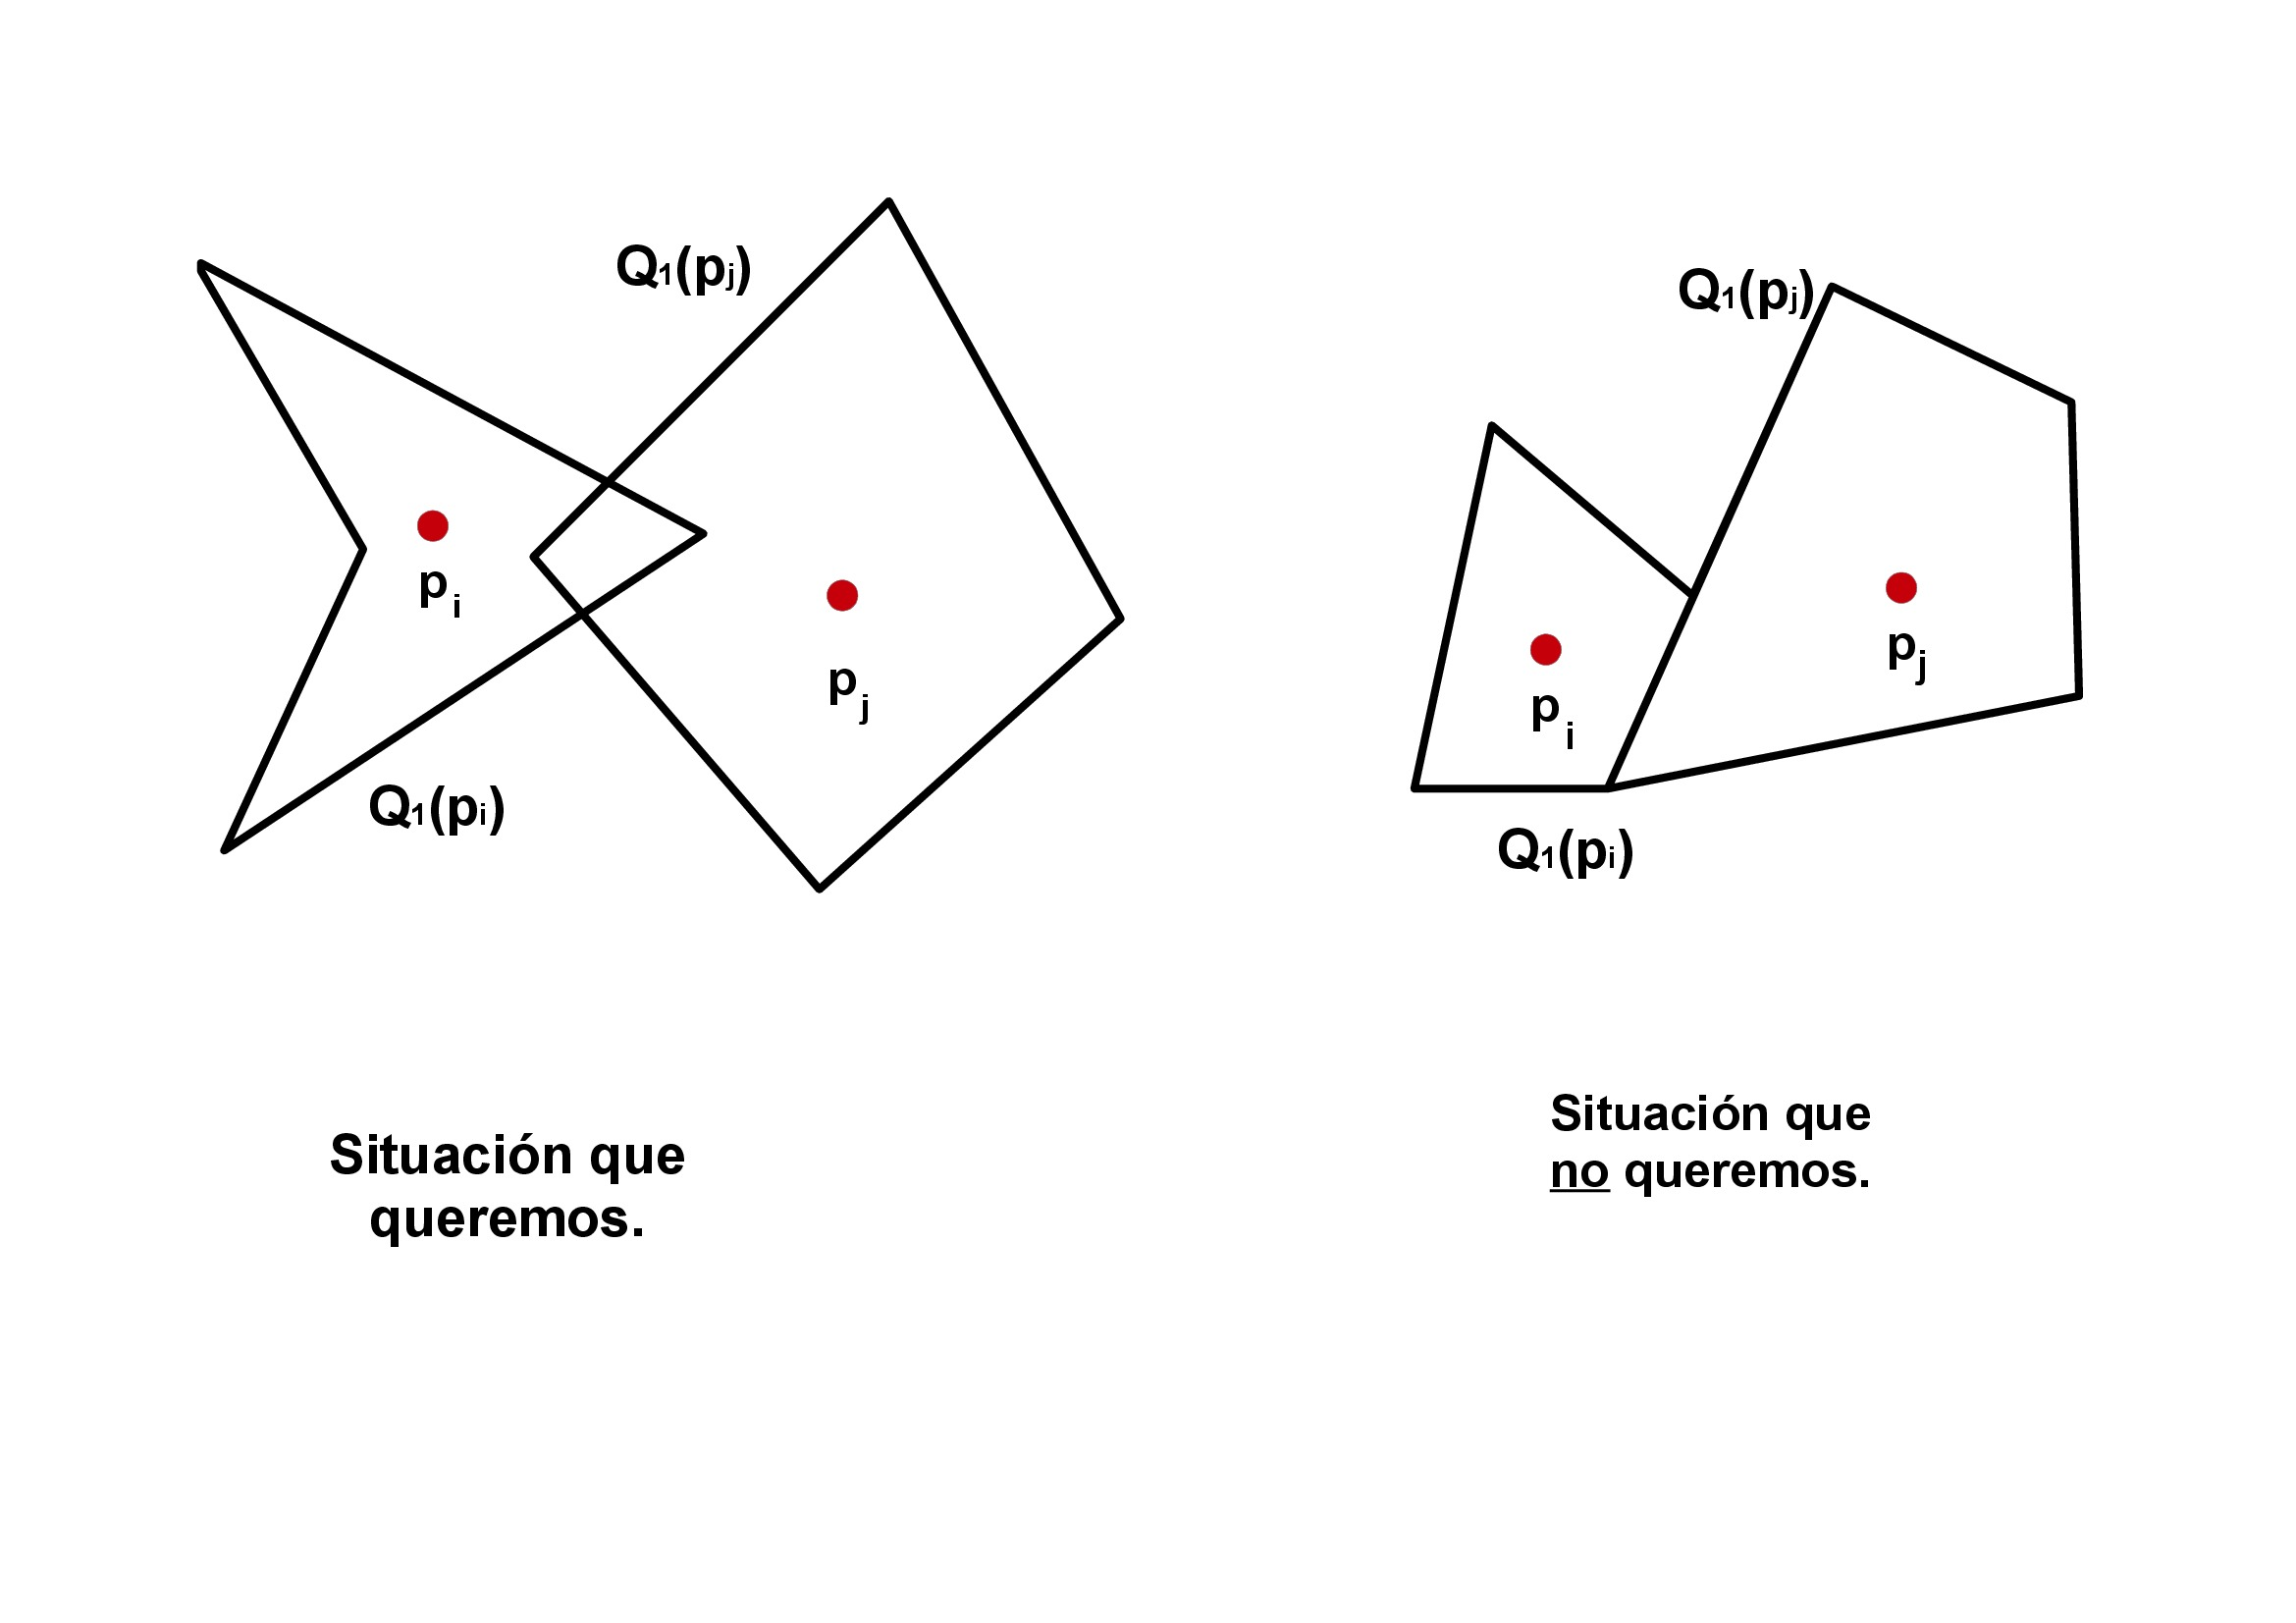
\includegraphics[width=10.0cm]{pic2.jpg}
        \end{minipage}
    \end{figure}
\end{frame}

\begin{frame}{Teorema de Radó}
    \begin{figure}[h]
    \centering
        \begin{minipage}[c]{\textwidth}
        \centering
        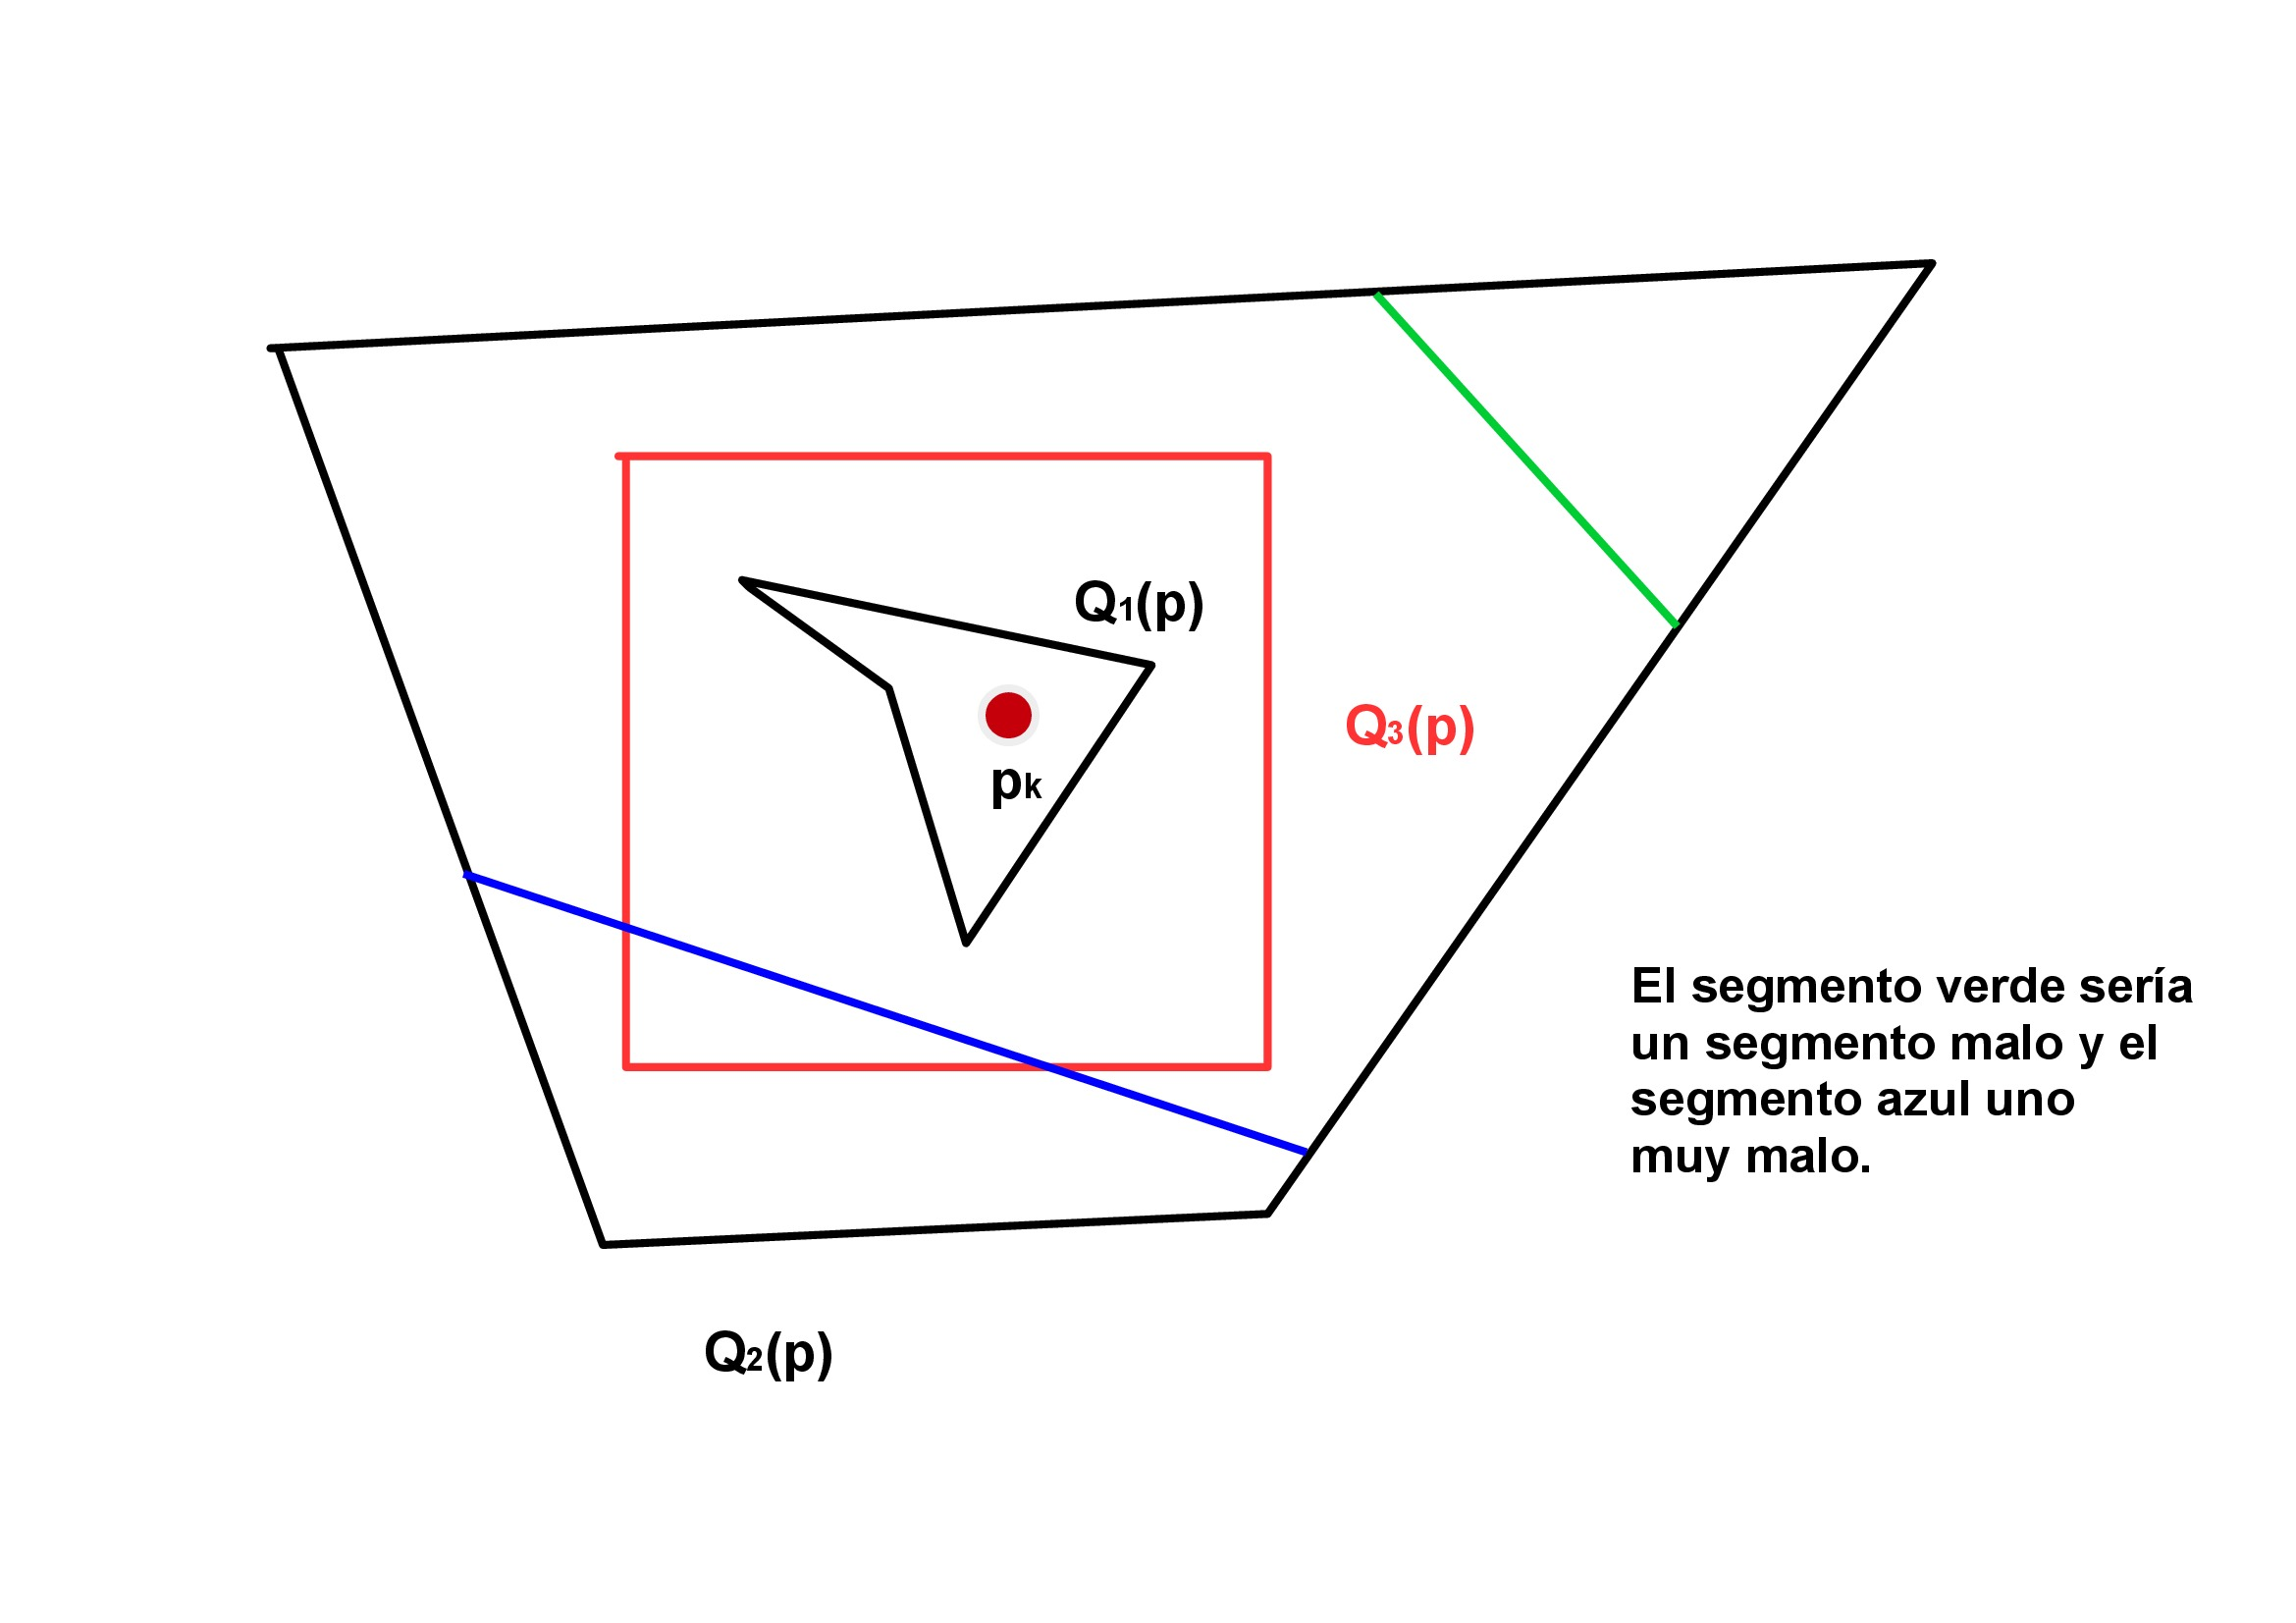
\includegraphics[width=10.0cm]{pic3.jpg}
        \end{minipage}
    \end{figure}
\end{frame}

\begin{frame}{Teorema de Radó}
    \begin{figure}[h]
    \centering
        \begin{minipage}[c]{\textwidth}
        \centering
        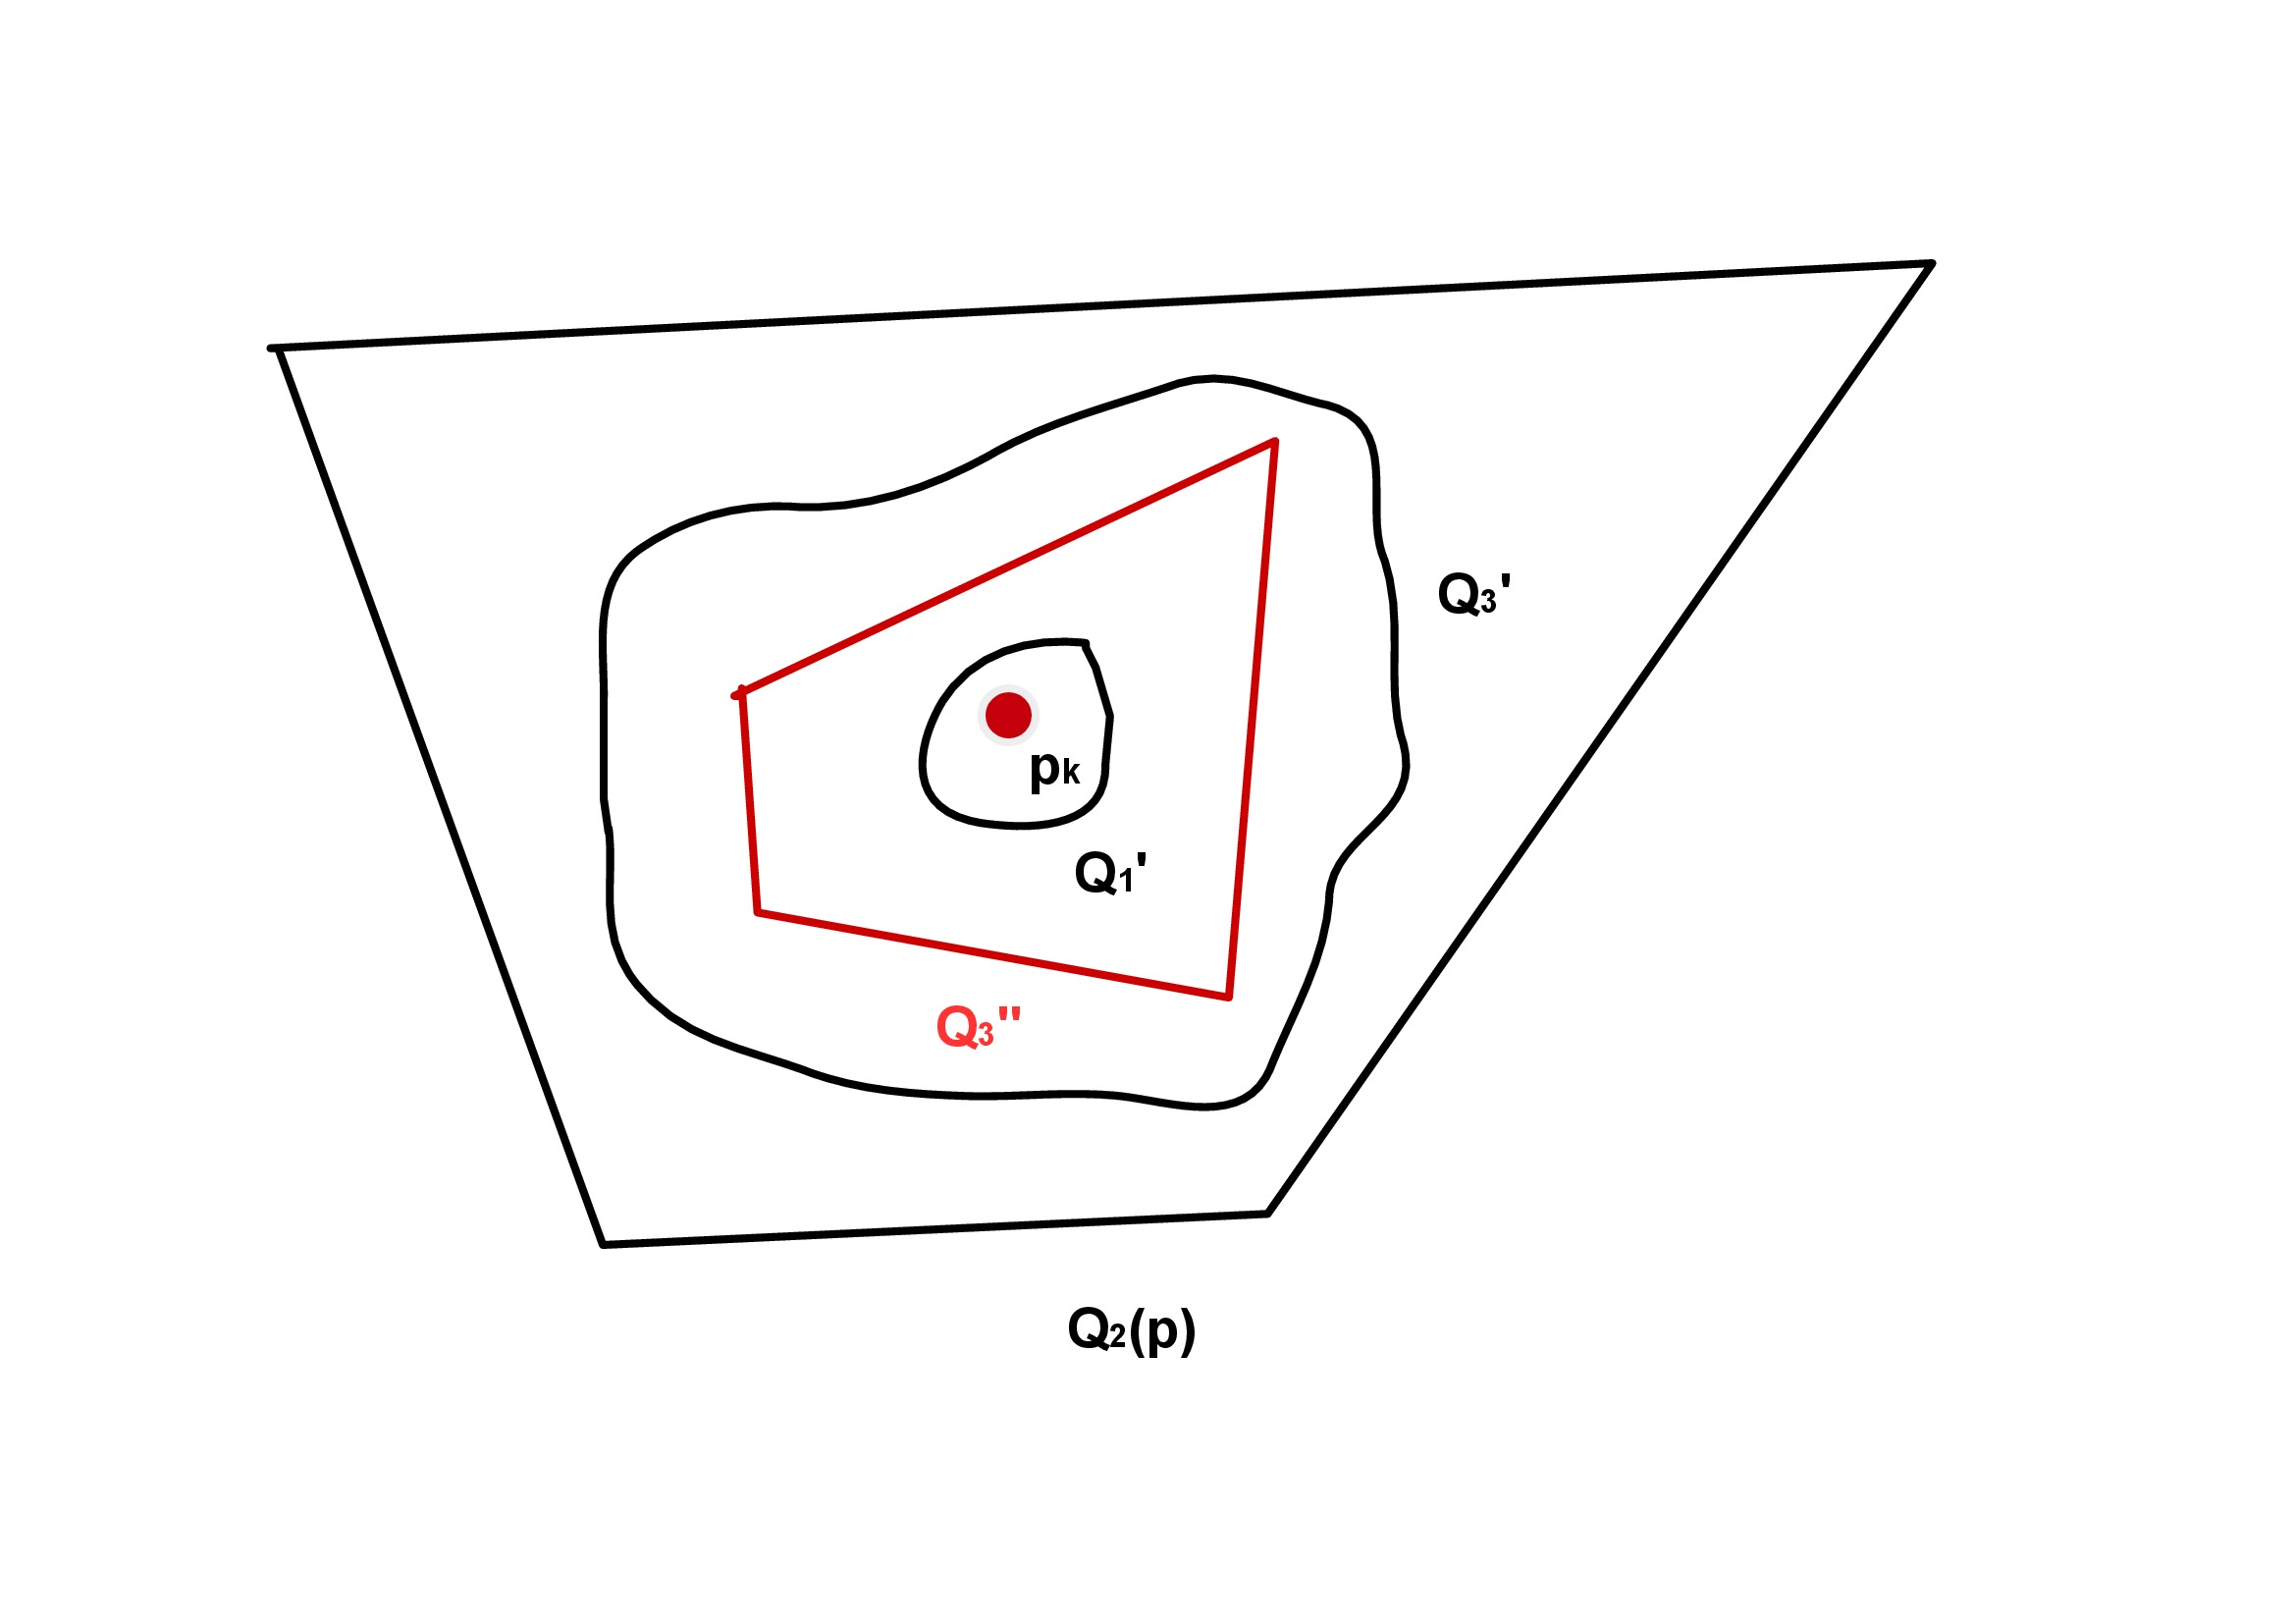
\includegraphics[width=10.0cm]{pic4.jpg}
        \end{minipage}
    \end{figure}
\end{frame}

\begin{frame}{Teorema de Radó}
    Como consecuencia directa del Teorema de Radó, toda superficie topológica compacta es homeomorfa a un polígono con lados identificados a pares. A partir de este hecho básico, y mediante métodos de cirugía topológica elemental, es posible demostrar que una superficie topológica compacta distinta de la esfera es homeomorfa a una suma conexa de toros o a una suma conexa de projectivos, siendo la unión de estas familias normalizadas de superficies exahustiva (esto es, no hay dos de ellas homeomorfas entre sí). Como corolario, toda superficie compacta se determina unívocamente por su característica de Euler y su carácter de orientabilidad.
\end{frame}

\appendix
\section<presentation>*{\appendixname}
\subsection<presentation>*{Referencias}

\begin{frame}
\frametitle<presentation>{Referencias}
\begin{thebibliography}{10}
    
	\beamertemplatearticlebibitems

	\bibitem{Thomassen}
	C. Thomassen
	\newblock The Jordan-Schönflies Theorem and the Classification of Surfaces, págs. 116-130
	\newblock American Mathematical Monthly, 1992
	
	\beamertemplatebookbibitems
	
	\bibitem{Massey}
	W. S. Massey
	\newblock {\em Algebraic Topology: An Introduction}
	\newblock Springer-Verlag, 1977
	
	\bibitem{Tutte}
    W. T. Tutte
    \newblock {\em Graph Theory}
    \newblock Addison Wesley, 1984
    
\end{thebibliography}
\end{frame}
    
\begin{frame}
\frametitle<presentation>{Referencias}
\begin{thebibliography}{10}
    \beamertemplatearticlebibitems
    
    \bibitem{Kuratowski}
	C. Thomassen
	\newblock Kuratowski's Theorem, págs. 225-241
	\newblock J. Graph Theory, 1981
	
	\bibitem{Stadler}
	M. M. Stadler
	\newblock ¿Qué es la Topología?
	\newblock Universidad del País Vasco-Euskal Herriko Unibertsitatea, 2002
	
	\beamertemplatebookbibitems
	
	\bibitem{Herrero}
	P. J. Herrero Piñeyro
	\newblock Topología de Espacios Métricos, págs. 9-18
	\newblock Universidad de Murcia, 2010
	
\end{thebibliography}
\end{frame}

\end{document}
